%-------------------------------------------------------------------------------
%	PACKAGES AND OTHER DOCUMENT CONFIGURATIONS
%-------------------------------------------------------------------------------

\documentclass[11pt]{article}

% Packages
% Packages

% \usepackage{fancyhdr} % Required for custom headers
% \usepackage{lastpage} % Required to determine the last page for the footer
% \usepackage{extramarks} % Required for headers and footers
% \usepackage[usenames,dvipsnames]{color} % Required for custom colors
\usepackage{graphicx} % Required to insert images
% \usepackage{listings} % Required for insertion of code
% \usepackage{courier} % Required for the courier font
% \usepackage{dsfont} % For special math characters
% \usepackage{verbatim}

%\usepackage{amsmath, amssymb, bm} % For matrix notation
\usepackage[english]{babel}
\usepackage[paperwidth=8.5in,paperheight=11in,margin=1.0in]{geometry}
\usepackage{listings}
\usepackage{hyperref}
%\usepackage[cmex10]{amsmath, bm}
\usepackage{amsmath, bm}
\usepackage{blkarray}








% formatting
\pdfcompresslevel0

% ==============================================================================
% PYTHON
% ==============================================================================
\usepackage[utf8]{inputenc}

% Default fixed font does not support bold face
\DeclareFixedFont{\ttb}{T1}{txtt}{bx}{n}{12} % for bold
\DeclareFixedFont{\ttm}{T1}{txtt}{m}{n}{12}  % for normal

% Custom colors
\usepackage{color}
\definecolor{deepblue}{rgb}{0,0,0.5}
\definecolor{deepred}{rgb}{0.6,0,0}
\definecolor{deepgreen}{rgb}{0,0.5,0}

\usepackage{listings}

% Python style for highlighting
\newcommand\pythonstyle{\lstset{
language=Python,
basicstyle=\ttm,
otherkeywords={self},             % Add keywords here
keywordstyle=\ttb\color{deepblue},
emph={MyClass,__init__},          % Custom highlighting
emphstyle=\ttb\color{deepred},    % Custom highlighting style
stringstyle=\color{deepgreen},
frame=tb,                         % Any extra options here
showstringspaces=false,            % 
breaklines=true
}}


% Python environment
\lstnewenvironment{python}[1][]
{\pythonstyle\lstset{#1}
}
{}

% Python for external files
\newcommand\pythonexternal[2][]{{
\pythonstyle\lstinputlisting[#1]{#2}}}

% Python for inline
\newcommand\pythoninline[1]{{\pythonstyle\lstinline!#1!}}
% ==============================================================================
% ==============================================================================

% Margins
\topmargin=-0.45in
\evensidemargin=0in
\oddsidemargin=0in
\textwidth=6.5in
\textheight=9.0in
\headsep=0.25in

\linespread{1.1} % Line spacing

% Set up the header and footer
\pagestyle{fancy}
\lhead{\hmwkAuthorName} % Top left header
\chead{\hmwkClass\ (\hmwkClassInstructor\ \hmwkClassTime): \hmwkTitle} % Top center head
\rhead{\firstxmark} % Top right header
\lfoot{\lastxmark} % Bottom left footer
\cfoot{} % Bottom center footer
\rfoot{Page\ \thepage\ of\ \protect\pageref{LastPage}} % Bottom right footer
\renewcommand\headrulewidth{0.4pt} % Size of the header rule
\renewcommand\footrulewidth{0.4pt} % Size of the footer rule

\setlength\parindent{0pt} % Removes all indentation from paragraphs

%----------------------------------------------------------------------------------------
%	DOCUMENT STRUCTURE COMMANDS
%	Skip this unless you know what you're doing
%----------------------------------------------------------------------------------------

% Header and footer for when a page split occurs within a problem environment
\newcommand{\enterProblemHeader}[1]{\nobreak\extramarks{#1}{#1 continued on next page\ldots}\nobreak\nobreak\extramarks{#1 (continued)}{#1 continued on next page\ldots}\nobreak}

% Header and footer for when a page split occurs between problem environments
\newcommand{\exitProblemHeader}[1]{\nobreak\extramarks{#1 (continued)}{#1 continued on next page\ldots}\nobreak\nobreak\extramarks{#1}{}\nobreak}

\setcounter{secnumdepth}{0} % Removes default section numbers
\newcounter{homeworkProblemCounter} % Creates a counter to keep track of the number of problems

\newcommand{\homeworkProblemName}{}
\newenvironment{homeworkProblem}[1][Problem \arabic{homeworkProblemCounter}]{ % Makes a new environment called homeworkProblem which takes 1 argument (custom name) but the default is "Problem #"
\stepcounter{homeworkProblemCounter} % Increase counter for number of problems
\renewcommand{\homeworkProblemName}{#1} % Assign \homeworkProblemName the name of the problem
\section{\homeworkProblemName} % Make a section in the document with the custom problem count
\enterProblemHeader{\homeworkProblemName} % Header and footer within the environment
}{\exitProblemHeader{\homeworkProblemName} % Header and footer after the environment
}

% Defines the problem answer command with the content as the only argument
\newcommand{\problemAnswer}[1]{\noindent\framebox[\columnwidth, resolution=600][c]{\begin{minipage}{0.98\columnwidth, resolution=600}#1\end{minipage}}}
% Makes the box around the problem answer and puts the content inside }

\newcommand{\homeworkSectionName}{}
\newenvironment{homeworkSection}[1]{ % New environment for sections within homework problems, takes 1 argument - the name of the section
\renewcommand{\homeworkSectionName}{#1} % Assign \homeworkSectionName to the name of the section from the environment argument
\subsection{\homeworkSectionName} % Make a subsection with the custom name of the subsection
\enterProblemHeader{\homeworkProblemName\ [\homeworkSectionName]} % Header and footer within the environment
}{
\enterProblemHeader{\homeworkProblemName} % Header and footer after the environment
}



%-------------------------------------------------------------------------------
%	NAME AND CLASS SECTION
%-------------------------------------------------------------------------------

\newcommand{\hmwkTitle}{HW 9} % Assignment title
\newcommand{\hmwkDueDate}{Tuesday, Oct. 20} % Due date
\newcommand{\hmwkClass}{Stat 860} % Course/class
\newcommand{\hmwkClassTime}{4:00 PM} % Class/lecture time
\newcommand{\hmwkClassInstructor}{Grace Wahba} % Teacher/lecturer
\newcommand{\hmwkAuthorName}{Elijah Bernstein-Cooper} % Your name

%-------------------------------------------------------------------------------
%	TITLE PAGE
%-------------------------------------------------------------------------------

\title{\vspace{0in}
    \textmd{\textbf{\hmwkClass:\ \hmwkTitle}}\\
    \normalsize\vspace{0.1in}\small{Due\ on\ \hmwkDueDate}\\
    \vspace{0.1in}\large{\textit{\hmwkClassInstructor\ \hmwkClassTime}}
    \vspace{0.2in}}

\author{\textbf{Elijah Bernstein-Cooper}}
\date{\today} % Insert date here if you want it to appear below your name

%-------------------------------------------------------------------------------

\begin{document}

\maketitle
%\newpage

%===============================================================================
%-------------------------------------------------------------------------------
%	PROBLEM 1
%-------------------------------------------------------------------------------
\begin{homeworkProblem}

    We compared the effects the peakedness of a function, the sampling size,
    and the noise have on the GCV estimate of a fitted cubic spline and the
    Bayesian confidence intervals of the fit. Figure 1 shows the GCV fit to
    low-noise peaky functions with different samplings. For a low number of
    samples, the spline smooths out the peak completely, however for a large
    number of samples, the spline is able to reproduce the peak. 91\% of data
    points are included within the Bayesian confidence intervals of the
    well-sampled peaky function (see Table 1). \\

    Figure 2 shows a comparison of spline fits to low-noise and high-noise
    smooth curves. We can see that the GCV estimate of the true function is
    accurate even in the high noise case because the function is smooth.\\

    Figure 3 shows a high-noise, high-sampling of the smooth curve. This shows
    a better estimate of the true function can either be obtained with a lower
    noise or a higher sampling. \\

    Finally, Table 1 shows the results from a variety of samplings and noises
    for the pointy and smooth functions. \\

    \begin{figure}[!ht]
        \begin{subfigure}{0.5\textwidth}
            \begin{centering}
                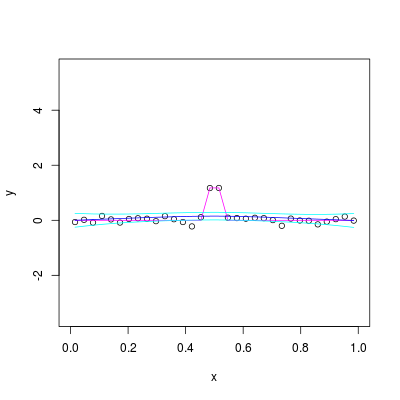
\includegraphics[width=\linewidth]{pointy_sig01_n32.png}
                \caption{$\sigma$ = 0.1, $n$ = 32}
            \end{centering}
        \end{subfigure}
        \begin{subfigure}{0.5\textwidth}
            \begin{centering}
                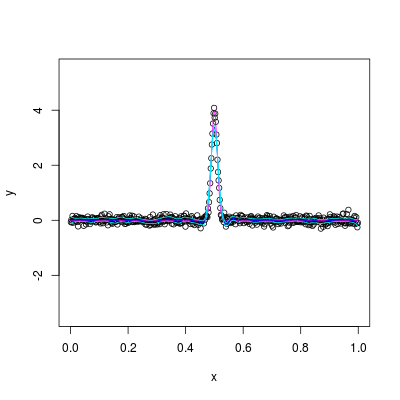
\includegraphics[width=\linewidth]{pointy_sig01_n512.png}
                \caption{$\sigma$ = 0.1, $n$ = 512}
            \end{centering}
        \end{subfigure}

        \caption{Plot showing true curve in magenta, noisy, discretely sampled
            curve as dots, the fitted GCV estimate of the noisy data, and the
            98\% confidence intervals shown in turquoise. }

    \end{figure}

    \begin{figure}[!ht]
        \begin{subfigure}{0.5\textwidth}
            \begin{centering}
                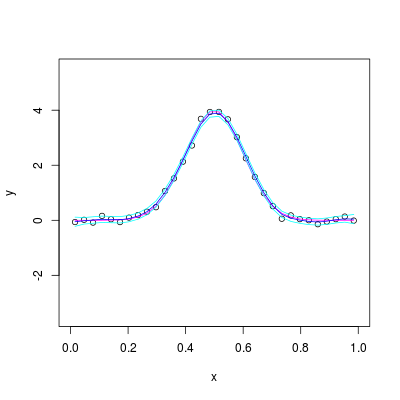
\includegraphics[width=\linewidth]{smooth_sig01_n32.png}
                \caption{$\sigma$ = 0.1, $n$ = 32}
            \end{centering}
        \end{subfigure}
        \begin{subfigure}{0.5\textwidth}
            \begin{centering}
                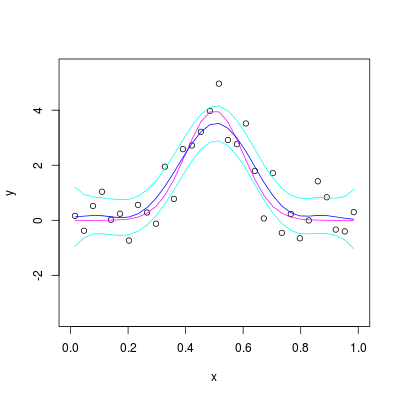
\includegraphics[width=\linewidth]{smooth_sig06_n32.png}
                \caption{$\sigma$ = 0.6, $n$ = 32}
            \end{centering}
        \end{subfigure}

        \caption{Plot showing true curve in magenta, noisy, discretely sampled
            curve as dots, the fitted GCV estimate of the noisy data, and the
            98\% confidence intervals shown in turquoise.}
    \end{figure}

    \begin{figure}[!ht]
        \begin{centering}
            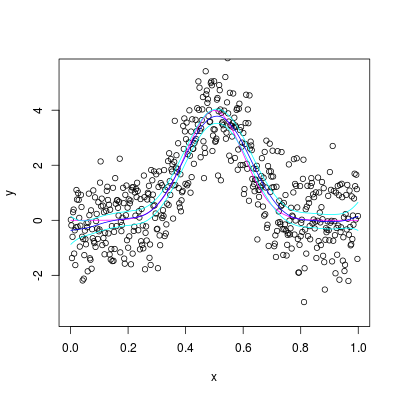
\includegraphics[width=0.5\linewidth]{smooth_sig1_n512.png}
            \caption{$\sigma$ = 1, $n$ = 512}
        \end{centering}
    \end{figure}

    \begin{table}[H]

        \caption{GCV Fitting Results}

        \begin{center}
            \begin{tabular}{lcc}

            Data properties & $\frac{\sigma_{\rm GCV}}{\sigma_{\rm true}}$ & \%
            Incl.
            \\ \hline \hline
            Pointy, $n = 32$, $\sigma = 0.1$ & 0.58 & 72 \\
            Pointy, $n = 512$, $\sigma = 0.1$ & 0.26 & 91 \\
            Pointy, $n = 32$, $\sigma = 1$ & 1.54 & 65 \\
            Pointy, $n = 512$, $\sigma = 1$ & 2.05 & 88 \\
            Smooth, $n = 32$, $\sigma = 0.1$ & 0.19 & 94 \\
            Smooth, $n = 512$, $\sigma = 0.1$ & 0.20 & 100 \\
            Smooth, $n = 32$, $\sigma = 1$ & 1.59 & 94 \\
            Smooth, $n = 512$, $\sigma = 1$ & 2.03 & 85 \\
            \hline
            \end{tabular}

            \vspace{1cm}

            \caption{$\frac{\sigma_{\rm GCV}}{\sigma_{\rm true}}$ is the ratio
                of the estimated to the true standard deviation, \% Incl.  is
                the fraction of data points included within the 98\% confidence
                intervals. We can see that for noisy or under-sampled data with
                a steep peak (the pointy data set), the fraction of data points
                within the confidence intervals is low. $\frac{\sigma_{\rm
                GCV}}{\sigma_{\rm true}}$ seems to depend only on the number of
                samples of the curve.}

        \end{center}
    \end{table}

    \begin{comment}

n = 32, pointy
nla gcvscore sigrat count
1.30972224290034 0.101536777192734 0.587433350073325 25
1.42378759312904 0.120404669999174 0.641741331904703 19
7.22872823697083 0.14359078357102 0.714233955273207 30
7.22781795298925 0.225169556803124 0.894400528152605 5
7.22863758374559 0.323244287395246 1.07162451414139 30
7.22760313985375 0.69346805863246 1.56960524649616 30
1.02253848075159 0.667217799800174 1.49106738174065 17
7.22835638881364 1.03626580577968 1.91872526547335 30
7.22938450333758 0.985848373124227 1.87146742686397 30
-0.250134734698906 0.834143707407556 1.54545861150742 21

n = 512, pointy
nla gcvscore sigrat count
-3.56067357117081 0.0205850291161235 0.268959052985345 467
-3.34329716331836 0.065018190249316 0.480058370748347 472
-3.15360299455419 0.121731067695499 0.660135943834066 469
-2.56367016963988 0.225966658841532 0.906208882997822 453
-2.56914632607116 0.400049942431737 1.20659042827437 449
-2.55792949149479 0.468894128796674 1.30557973159123 463
-2.23310281179193 0.610945656899442 1.49979644243047 465
-2.57205032394069 0.809242800871517 1.71979111575181 471
-2.56708636717109 0.940375239947086 1.85467438843456 480
-2.57237280310689 1.15419592565096 2.05121307538029 453
average count = 464.2

n = 32, smooth
nla gcvscore sigrat count
-1.98587376402231 0.0272268862669426 0.196889596885868 30
-1.38254479686723 0.132340539377237 0.521640608570361 28
-1.58739846027184 0.142063867826474 0.515401449188675 32
-1.33847430644458 0.228736007703634 0.695260123608778 24
-0.934740231203872 0.36704927829582 0.947150111102719 22
-0.852758816020283 0.923884800661332 1.52110341907422 32
-0.82514201520053 0.693446140663359 1.32101091521949 23
-0.775794592274177 1.34367057547859 1.85261225482618 32
-0.212600928631447 1.35117279436996 1.97444904408382 24
-1.04338346776945 1.06668556360459 1.58504841527458 26
average count = 27.3

n = 512, smooth
nla gcvscore sigrat count
-1.47169557443604 0.0109955851930503 0.203437433389029 512
-1.20835676059262 0.0447023964722302 0.411937810056396 461
-1.14375858539518 0.10022900379521 0.617794983485965 512
-0.834554305147125 0.157391797454557 0.776055186694482 489
-1.11728784505647 0.262915009990858 1.00008989847503 503
-0.664491988319057 0.365980286286347 1.18574285360294 512
-0.628474351594141 0.515310852294453 1.40745900191405 512
-0.412246522886022 0.702770517196645 1.64781465834901 456
-0.402426967020027 0.786052648578202 1.74251189160877 461
-0.374979977644127 1.06244972493778 2.02669125746893 435
average count = 485.3

    \end{comment}


\end{homeworkProblem}
%===============================================================================

\end{document}

